\section{Building a high--fidelity processor}
\label{sec:processor}
%%%%%%%%%%%%%%%%%%%%%%%%%%%%%%%%%%%%%%%%%%%%%%%%%%%%%%%%%%%%%%%%%%%%%%%%%%%%%%%%%%%%%%%%%%%%%%%%%
%
% The following paragraph contains an example of an internal reference. Use the
% command \ref{•} along with the identifier defined with the command \label{•} to create
% a reference to an internal section on your research paper. The label can be defined in
% any of the .tex files that you have included.
%
%%%%%%%%%%%%%%%%%%%%%%%%%%%%%%%%%%%%%%%%%%%%%%%%%%%%%%%%%%%%%%%%%%%%%%%%%%%%%%%%%%%%%%%%%%%%%%%%%
We designed a quantum processor named ``Sycamore'', shown in
Figure~\ref{fig:sycamore_processor}, which consists of a two--dimensional array
of 54 transmon qubits, where each qubit is tunably coupled to four nearest
neighbors, in a rectangular lattice.

%%%%%%%%%%%%%%%%%%%%%%%%%%%%%%%%%%%%%%%%%%%%%%%%%%%%%%%%%%%%%%%%%%%%%%%%%%%%%%%%%%%%%%%%%%%%%%%%%
%
% The following paragraph contains several examples:
%
%   1.- A figure. Use the environment \begin{figure} ... \end{figure} to insert
%       an image.
%
%   2.- Centering in the page. Use the command \centering to center horizontally
%       in the page
%
%   3.- Define the image to insert. Use the command \includegraphics[scale=•]{•}
%       to select the image to be inserted. Change the size of the image with the
%        scale parameter and provide the relative path to the image.
%
%   4.- Create a caption for the image. Use the command \caption{•} to include an 
%       explanatory text of the image. Be as self-contained as possible.
%
%   5.- Math mode. Use the characters $ $ to enclose a math mode section within
%       your text.
%
%   6.- Definition of the label. Use the command \label{•} to be used/referenced in
%       a different section of your research paper.
%
%%%%%%%%%%%%%%%%%%%%%%%%%%%%%%%%%%%%%%%%%%%%%%%%%%%%%%%%%%%%%%%%%%%%%%%%%%%%%%%%%%%%%%%%%%%%%%%%%
\begin{figure}[t]
  \centering
  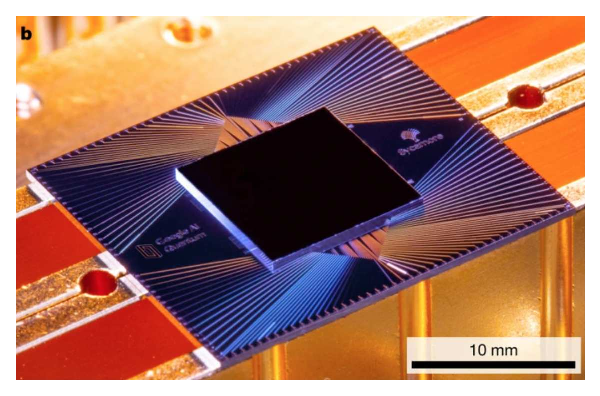
\includegraphics[scale=0.8]{img/sycamore.pdf}
  \caption{Photograph of the Sycamore chip.}
  \label{fig:sycamore_processor}
\end{figure}

...

...

...

%%%%%%%%%%%%%%%%%%%%%%%%%%%%%%%%%%%%%%%%%%%%%%%%%%%%%%%%%%%%%%%%%%%%%%%%%%%%%%%%%%%%%%%%%%%%%%%%%
%
% The following paragraph contains an example of a bullet list. Use the
% environment \begin{itemize} ... \end{itemize} to produce an itemized/bullet
% list. Each bullet is defined with the command \item 
%
%%%%%%%%%%%%%%%%%%%%%%%%%%%%%%%%%%%%%%%%%%%%%%%%%%%%%%%%%%%%%%%%%%%%%%%%%%%%%%%%%%%%%%%%%%%%%%%%%
The qubit is encoded as the two lowest quantum eigenstates of the resonant
circuit. Each transmon has two controls:

\begin{itemize}
  \item  A microwave drive to excite the qubit, and
  \item A magnetic flux control to tune the frequency.
\end{itemize}

Each qubit is connected to a linear resonator ...

...